\chapter{Portraits de phases de systèmes non-linéaires}
    \section{Introduction}
    \section{Systèmes non-linéaires d'ordre 2}
        Soit un système dynamique non-linéaire défini par le système d'équations différentielles :
        \begin{equation}
            \begin{cases}
                \dot{x}_1 = f_1(x_1, x_2) \\
                \dot{x}_2 = f_2(x_1, x_2)
            \end{cases}
        \end{equation}
        où au moins une des fonctions $f_1$ ou $f_2$ est non linéaire. Dans le cas de systèmes non linéaires, l'analyse directe peut être complexe, voire impossible. Cependant, une approche standard pour comprendre le comportement local du système autour d'un point d'équilibre consiste à linéariser le système. Cette méthode s'appuie sur le développement de la fonction au voisinage de points spécifiques (typiquement des points d'équilibre) et permet d'extraire des informations cruciales sur la dynamique locale.

        Pour réaliser cette approximation linéaire, pour autant que $f_1$ et $f_2$ sont dérivables, nous calculons la \textit{matrice jacobienne} du système, qui décrit la variation infinitésimale des fonctions $f_1$ et $f_2$ par rapport aux variables $x_1$ et $x_2$. Renvoyons bien entendu l'étudiant·e au cours de Mathématiques pour une définition formelle de la dérivabilité (\cite{mathf117}). La matrice jacobienne s'exprime comme suit :

        \begin{definition}{Matrice jacobienne}
            La matrice jacobienne d'un système est définie comme la matrice des dérivées partielles selon les composantes. Dans le cas d'ordre 2,
            \begin{equation}
                J = 
                \begin{bmatrix}
                    \pd {f_1}{x_1} & \pd {f_1}{x_2} \\
                    \pd {f_2}{x_1} & \pd {f_2}{x_2}
                \end{bmatrix}
            \end{equation}
        \end{definition}
        L'évaluation de cette matrice au point d'équilibre (en posant $\dot{x}_1 = \dot{x}_2 = 0$) fournit un système linéarisé, dont le comportement global autour de l'équilibre peut être interprété en analysant les valeurs propres de $J$.

        Les valeurs propres de cette matrice jacobienne jouent un rôle crucial dans la classification locale du point d'équilibre en tant que nœud, foyer, point-selle, ou centre :
        \begin{itemize}
            \item si les valeurs propres sont réelles et de même signe, le point d'équilibre est un nœud attractif ou répulsif~;
            \item si les valeurs propres sont réelles et de signes opposés, le point d'équilibre est un point-selle, indiquant un comportement divergent sur certaines directions et convergent sur d'autres~;
            \item si les valeurs propres sont complexes conjuguées avec une partie réelle non nulle, le point est un foyer, décrivant un comportement oscillatoire autour de l'équilibre~;
            \item si les valeurs propres sont purement imaginaires, le point d'équilibre est un centre, et le système suit des trajectoires fermées autour de ce point.
        \end{itemize}
        Notons que cette classification est uniquement valide si les valeurs propres de $J$ sont toutes deux non nulles, assurant que le point d'équilibre est non dégénéré.

        \subsection{Calcul des isoclines}
            Le calcul des isoclines d'un système non-linéaire se fait de manière analogue à celle des cas linéaire. La définition d'une isocline (voir \ref{def:isocline}) reste valable: pour calculer les isoclines d'un système, on détermine l'équation obtenue par l'annulation de chacune des dérivées. Prenons par exemple le système
            \begin{equation}\label{eq:isocline_non_lineaire}
                \begin{cases}
                    \dot{x}_1 = x_1^2 + x_2 \\
                    \dot{x}_2 = x_2
                \end{cases}
            \end{equation}

            Nous pouvons en calculer les deux isoclines. Commençons par annuler la première dérivée. L'isocline correspondante est décrite par l'équation $0 = x_1^2 + x_2$, ou $x_2 = -x_1^2$. C'est une équation parabolique négative dont le sommet se trouve à l'origine. La deuxième isocline se calcule de manière similaire, et donne $x_2 = 0$, droite horizontale confondue avec l'axe $x_1$. Dans la figure \ref{}, on montre le portrait de phase associé à ce système.
            \begin{figure}[ht!]
                \centering
                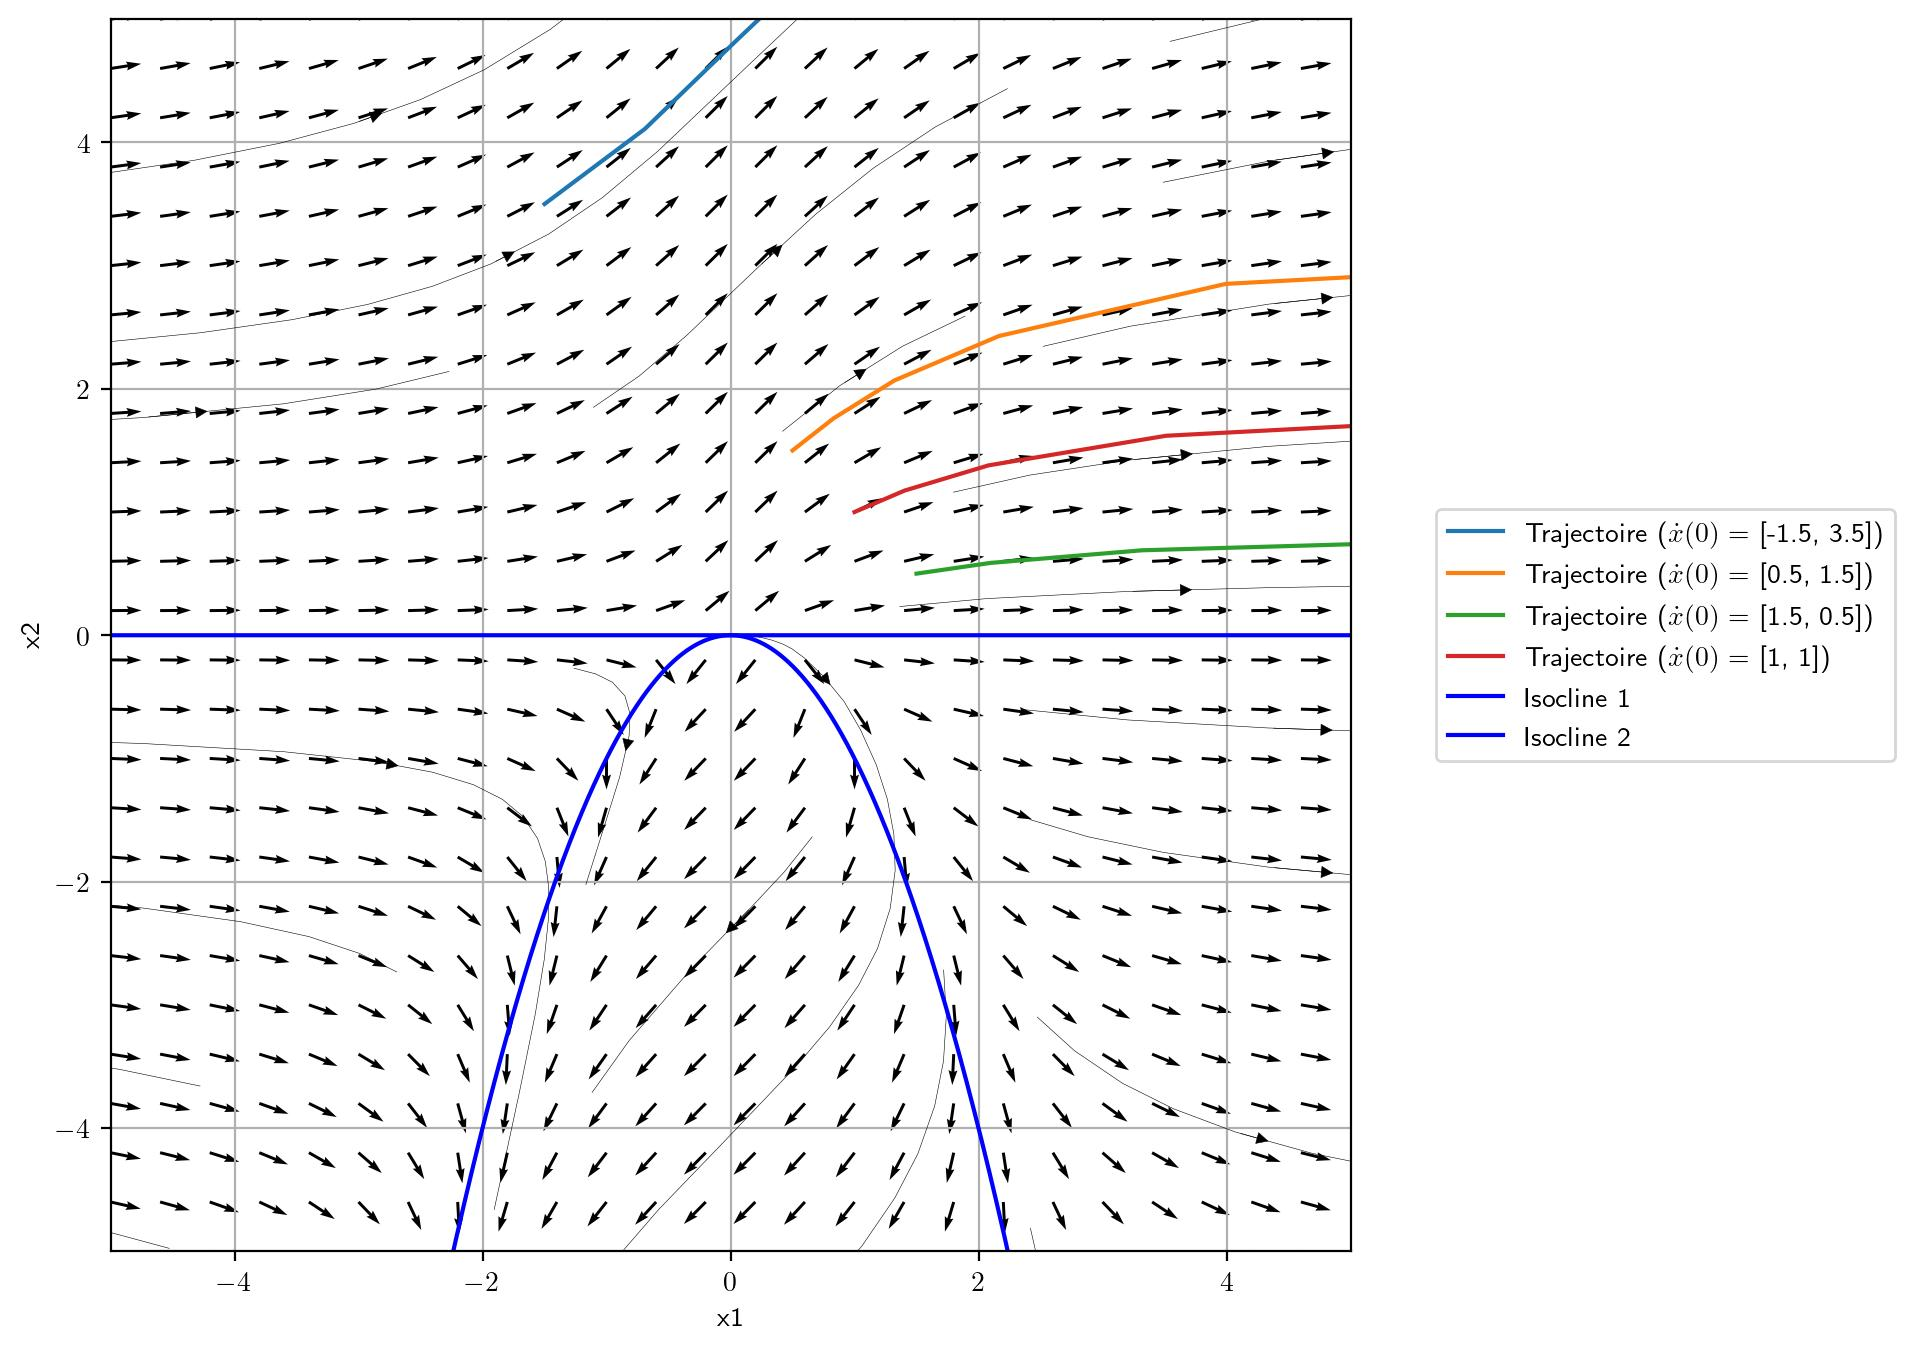
\includegraphics[width=\textwidth]{images/exemple_non_lineaire_1.jpg}
                \caption{Portrait de phase du système \ref{eq:isocline_non_lineaire}. Les deux isoclines sont marquées en bleu.}
                \label{fig:exemple_non_lineaire_1}
            \end{figure}

        \subsection{Calcul des points d'équilibre}
            Ici encore, la définition donnée en \ref{def:point_equilibre} reste valable: les points d'équilibres sont les points pour lesquels la variation est nulle (c'est à dire, où les deux dérivées sont annulées en même temps). Par définition, les points d'équilibre correspondent aux points d'intersection entre les isoclines.
            Prenons le système
            \begin{equation}\label{eq:equilibre_non_lineaire}
                \begin{cases}
                    \dot{x}_1 = x_1 \\
                    \dot{x}_2 = \sin{x_2}
                \end{cases}
            \end{equation}
            Calculer le (les) point(s) d'équilibre revient à résoudre le système
            \begin{equation}
                \begin{cases}
                    0 = x_1 \\
                    0 = \sin{x_2}
                \end{cases}
            \end{equation}
            Les points d'équilibre sont donc situés sur la droite d'équation $x_1 = 0$, là ou $\sin x_2 = 0$. La figure \ref{fig:equilibre_non_lineaire_2} montre le portrait de phase associé au système \ref{eq:equilibre_non_lineaire} et en montre les points d'équilibre.
            \begin{figure}[ht!]
                \centering
                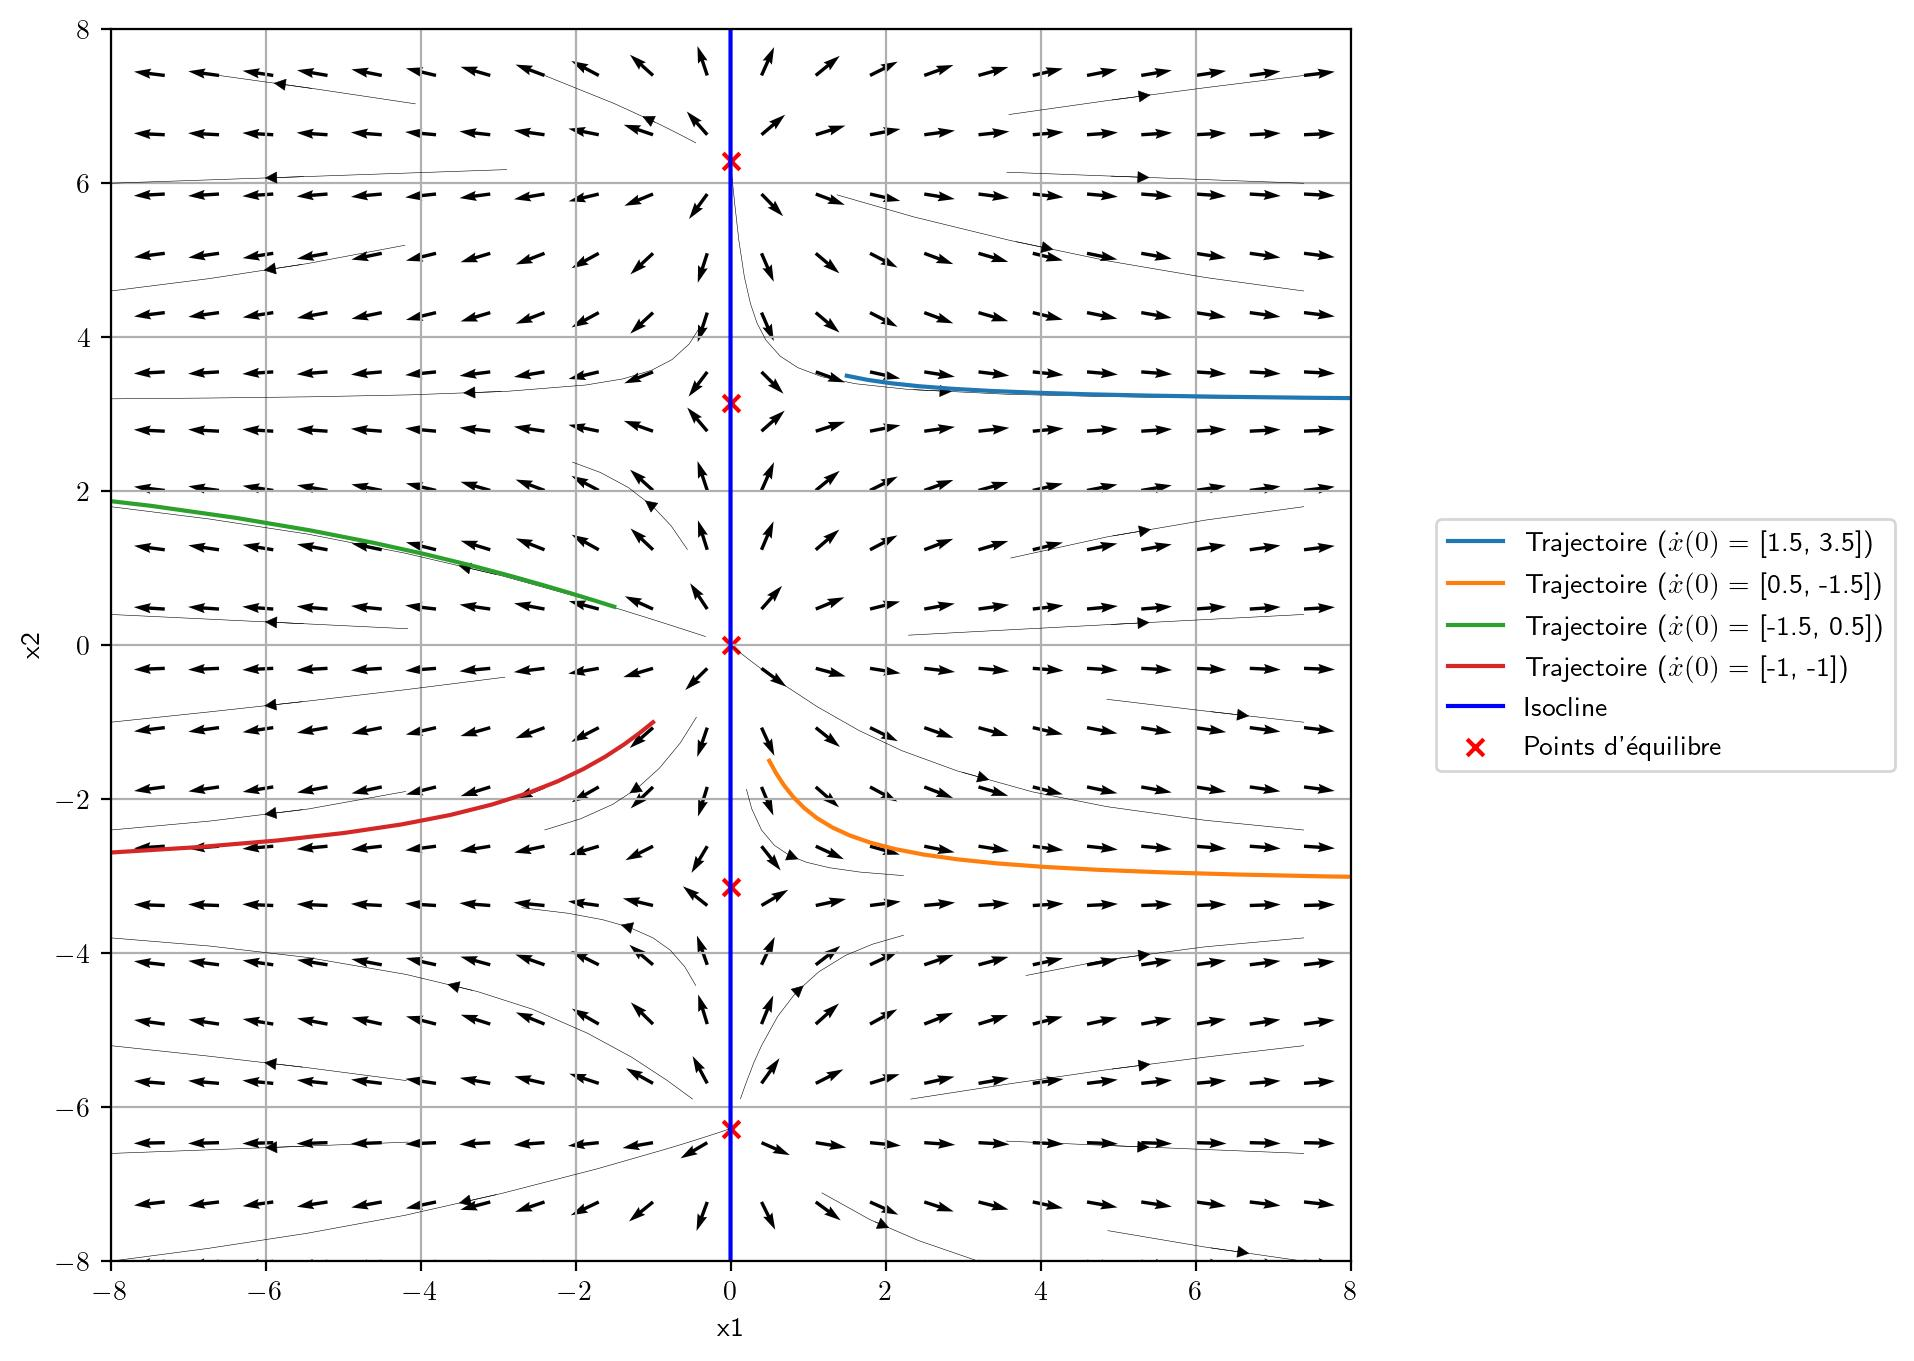
\includegraphics[width=\textwidth]{images/exemple_non_lineaire_2.jpg}
                \caption{Portrait de phase du système \ref{eq:equilibre_non_lineaire}. Les points d'équilibre sont marqués par des croix rouges.}
                \label{fig:equilibre_non_lineaire_2}
            \end{figure}
            
        \subsection{Stabilité des points d'équilibre}
            Le système précédent met en avant un phénomène déjà étudié dans le cadre des systèmes linéaires, celui de \textit{stabilité}. 
            Autour des différents points d'équilibre montrés sur dans la figure \ref{fig:equilibre_non_lineaire_2}, les trajectoires et les vecteurs vitesse s'éloignent, montrant qu'une condition initiale proche du point d'équilibre aura tendance à mener à une trajectoire divergente de ce point. Ces points d'équilibres sont donc \textit{instables}. Formellement, les définitions données en \ref{def:stabilite} restent valables dans le contexte non-linéaire, bien que leur vérification puisse demander des calculs plus fastidieux. En effet, comme expliqué dans le syllabus (\cite{infof305}), la vérification de la stabilité des points d'équilibre peut être réalisée en étudiant les \textit{critères de stabilité de Lyapounov\footnote{Alexandre Lyapounov (en russe, Александр Михайлович Ляпунов est un mathématicien russe né en 1857 et mort de sa propre main en 1918. Ses contributions majeurs concernent l'étude de la stabilité des systèmes dynamiques. Ce sujet vaste trouve ses balbutiements au 17ème siècle, avec des mathématiciens comme Evangelisto Torricelli et Galileo Galilei.}} (\cite{lyapounov}). 

            Pour rappel: soit un système à temps continu décrit par $\dot{x}(t) = f(x(t), u(t))$, où $f(\cdot, \cdot)$ et ses dérivées partielles sont connues. Admettons que nous ayons déjà calculé les points d'équilibre, comme expliquée dans la section précédente, et soit un point d'équilibre $\bar{x}$. Lyapounov nous dit que si il existe une fonction $V(\cdot)$ continue, ainsi que ses dérivées partielles, qui est définie positive en $\bar{x}$ et telle que la fonction 
            \begin{equation}
                \dot{V}(x(t)) = \frac{\dd V(x(t))}{\dd t} = \nabla V(x)f(x, \bar u)
            \end{equation}
            où $\nabla V(x) = [\frac{\dd V}{\dd x_1}, \frac{\dd V}{\dd x_2}, ..., \frac{\dd V}{\dd x_n}]$, est semi-définie négative en $\bar x$ alors $\bar x$ est un état d'équilibre \textit{stable}. Si cette même fonction est définie négative, alors l'équilibre est \textit{asymptotiquement stable}.

            Afin de rendre ces définitions plus claires, reprenons le système \ref{eq:equilibre_non_lineaire} en exemple:
            \begin{equation}
                \begin{cases}
                    \dot{x}_1 = x_1 \\
                    \dot{x}_2 = \sin{x_2}
                \end{cases}
            \end{equation}
            Nous avons déjà calculé ses points d'équilibre, prenons l'origine comme cas étudié ici.

            Prenons une fonction de Lyapounov candidate (et effectivement définie positive:
            \begin{equation}
                V(x_1, x_2) = \frac12 x_1^2 + \frac12 x_2² + 1
            \end{equation}
            Son gradient le long des trajectoires du système est donné par 
            \begin{equation}
                \dot V(x_1, x_2) = x_1x_1 + x_2\sin x_2 = x_1^2 + x_2\sin x_2
            \end{equation}
            Étudions le signe de cette fonction. Le premier terme, $x_1^2$ est positif ou nul. Rappelons que le point d'équilibre est à l'origine. Si $x_2$ est (donc légèrement) négatif, son sinus l'est aussi, et le deuxième terme est positif. Si $x_2$ est légèrement positif, son sinus l'est aussi et le deuxième terme est aussi positif. Le résultat de cette expression est donc positif dans le voisinage du point d'équilibre. Si l'on reprend le critère de Lyapounov, il en résulte que $V(\cdot)$ n'est ni définie négative, ni semi-définie négative, donc le système n'est pas stable. En se référant à la définition d'instabilité du syllabus, on en déduit que le système est instable autour de ce point d'équilibre. Observons à nouveaux le portrait de phase donné en figure \ref{fig:equilibre_non_lineaire_2}. Le point d'équilibre à l'origine semble en effet instable.
            
    \section{Exercices}
        L’objectif est de mener une analyse complète de ces systèmes en plusieurs étapes, qui sont détaillées ci-dessous. Cette analyse permettra d’examiner la dynamique des solutions dans le plan de phase et d’approfondir notre compréhension des comportements locaux autour des points d'équilibre.
    
        \begin{enumerate}
            \item Calcul et tracé des isoclines.
            \item Détermination des points d'équilibre
            \item Calcul de la matrice jacobienne. Le calcul de $J$ pour chacun des systèmes aux points d’équilibre permet d'obtenir une approximation linéaire du comportement du système autour de ces points.
            \item Étude du comportement local avec la matrice jacobienne: au voisinage de chaque point d’équilibre, nous utilisons la matrice jacobienne pour analyser la stabilité locale, comme vu durant ce chapitre. En examinant les valeurs propres de cette matrice, nous déterminons la nature du point d'équilibre (nœud, foyer, point-selle, etc.) et décrivons le comportement local des trajectoires.
            \item Dessin du portrait de phase.
            \item Étude analytique, par une fonction de Lyapounov bien choisie, de la stabilité des points d'équilibre, comme montré dans ce chapitre.
            
        
        \end{enumerate}
        Cette démarche permet une compréhension approfondie de chaque système dynamique, tant au niveau local qu’au niveau global, en combinant linéarisation locale et analyse graphique pour obtenir une interprétation complète des trajectoires et des comportements des solutions.

        \subsection{Exercice 1}
            \begin{exercise}{Exercice 1}
                \begin{equation}
                    \begin{cases}
                        \dot{x}_1 = x_1 \\
                        \dot{x}_2 = x_1^2 + x_2^2 - 1
                    \end{cases}
                \end{equation}
            \end{exercise}
            La solution numérique est donnée à titre indicatif dans la figure \ref{fig:pdp_exercice_3_1}.
            \begin{figure}[ht!]
                \centering
                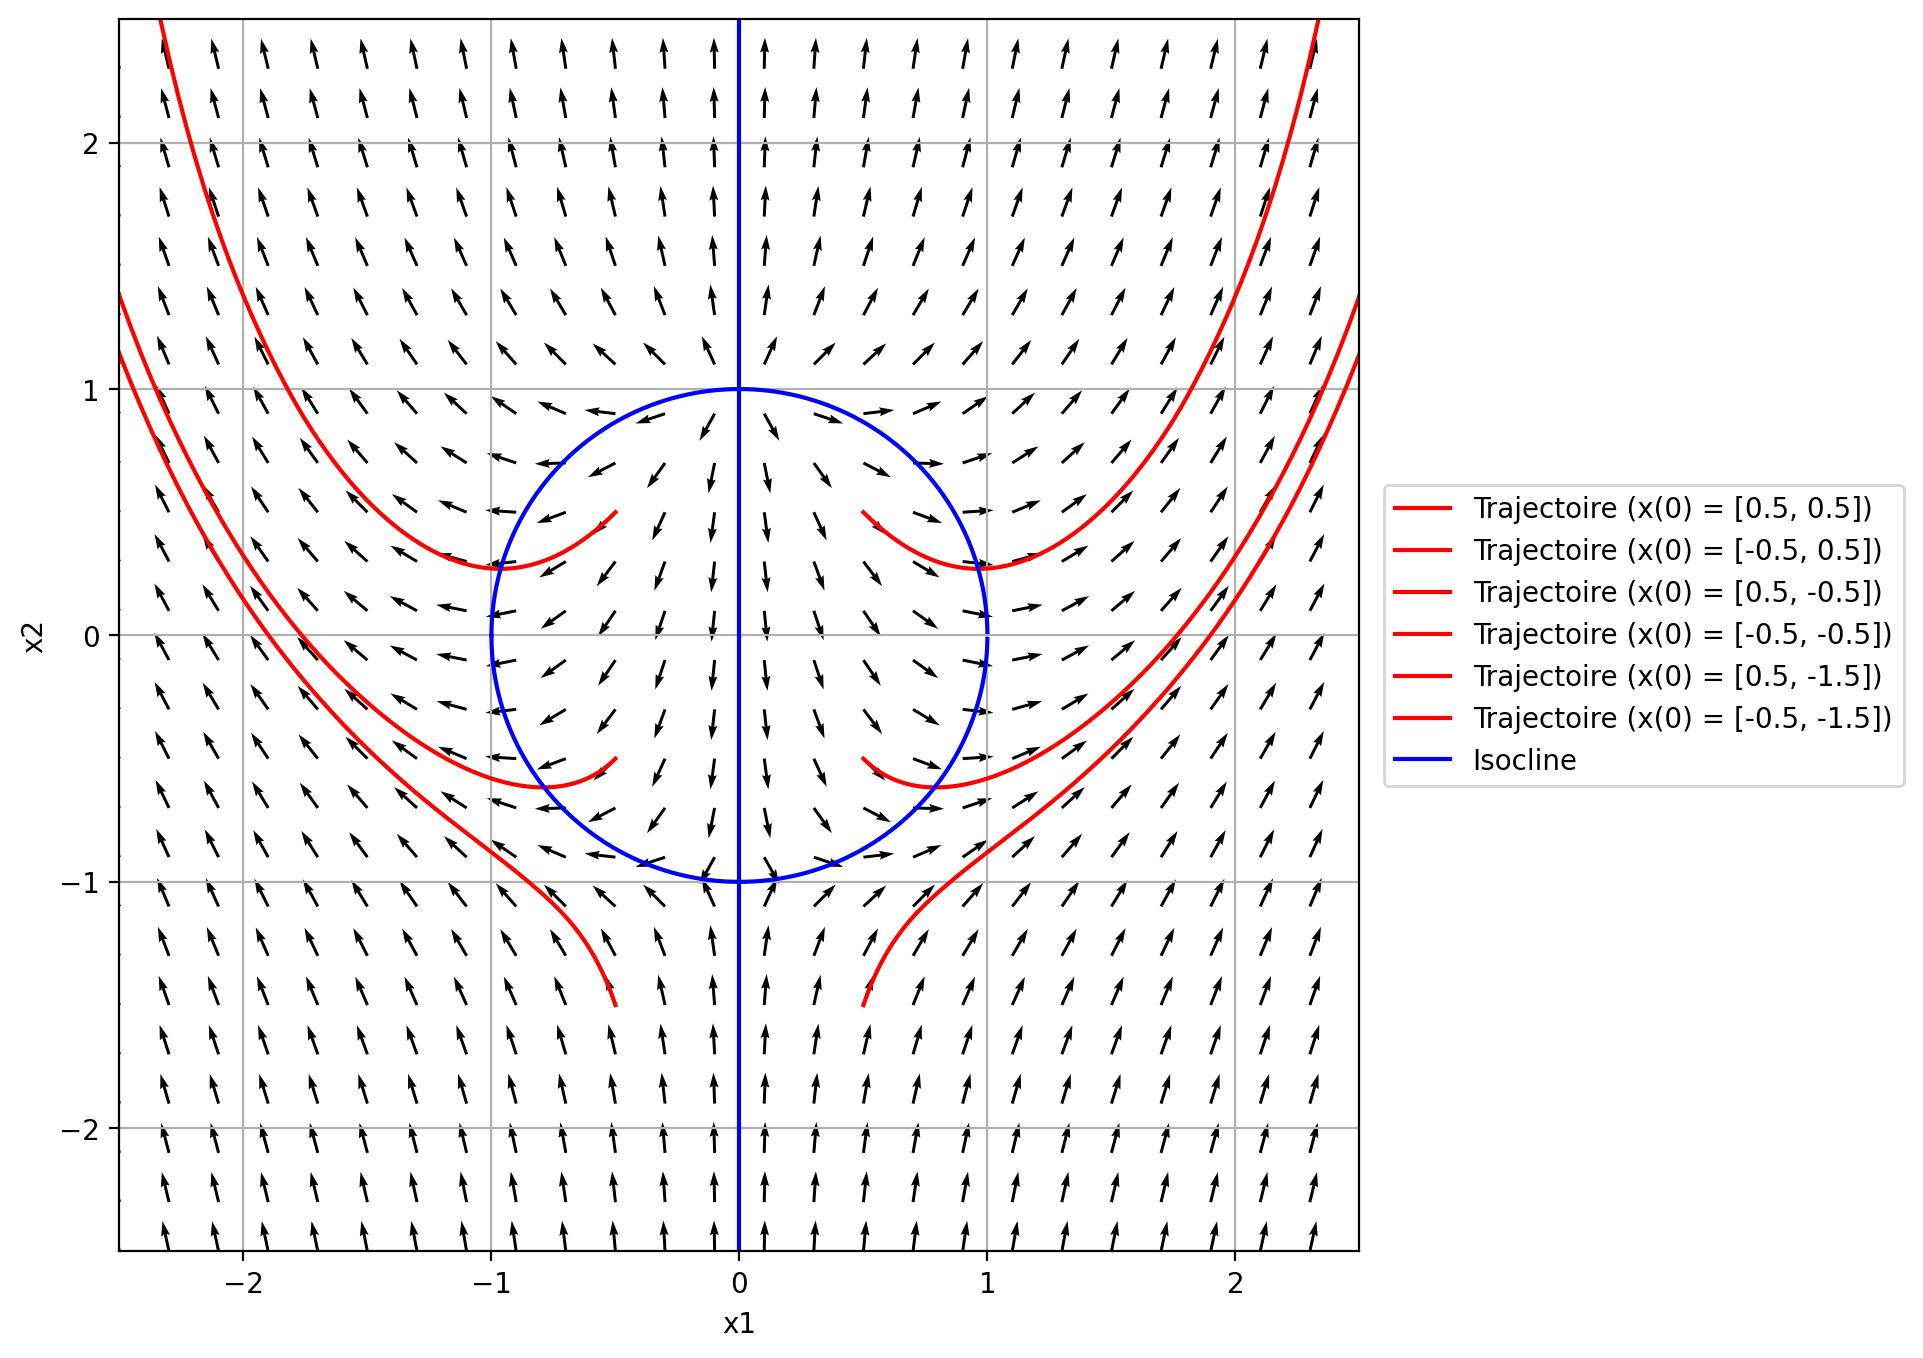
\includegraphics[width=\textwidth]{images/pdp_exercice_3_1.jpg}
                \caption{Solution numérique de l'exercice 1}
                \label{fig:pdp_exercice_3_1}
            \end{figure}
            
        \subsection{Exercice 2}
            \begin{exercise}{Exercice 2}
                \begin{equation}
                    \begin{cases}
                        \dot{x}_1 = x_2 \\
                        \dot{x}_2 = x_1(1 - x_1^2) + x_2
                    \end{cases}
                \end{equation}
            \end{exercise}
            La solution numérique est donnée à titre indicatif dans la figure \ref{fig:pdp_exercice_3_2}.
            \begin{figure}[ht!]
                \centering
                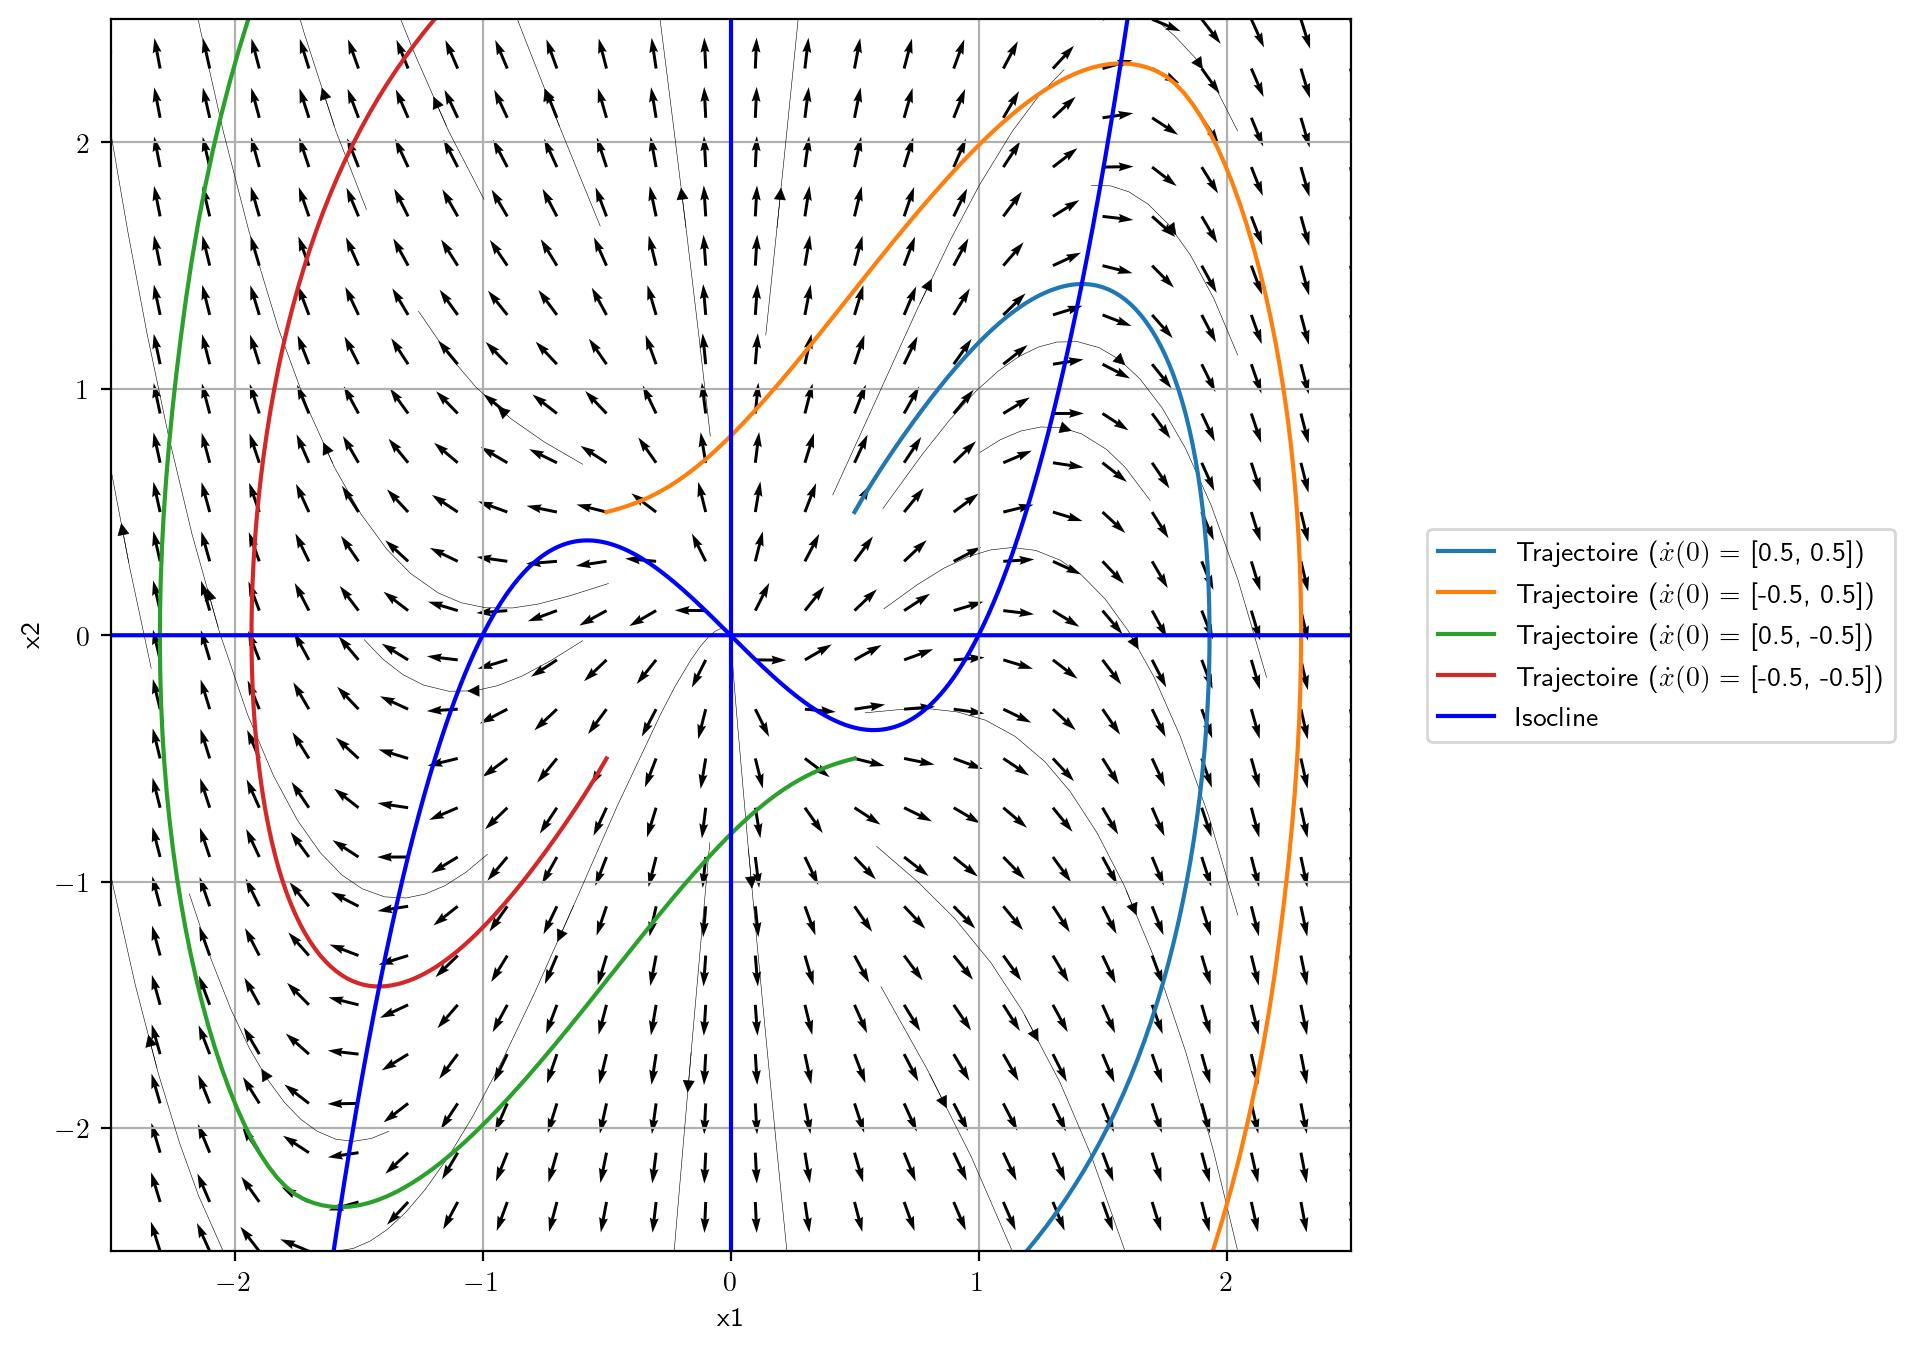
\includegraphics[width=\textwidth]{images/pdp_exercice_3_2.jpg}
                \caption{Solution numérique de l'exercice 2}
                \label{fig:pdp_exercice_3_2}
            \end{figure}

        \subsection{Exercice 3}
            \begin{exercise}{Exercice 3}
                \begin{equation}
                    \begin{cases}
                        \dot{x}_1 = 0.2 x_1 - 0.08 x_1 x_2 \\
                        \dot{x}_2 = 0.1 x_1 x_2 - 0.2 x_2
                    \end{cases}
                \end{equation}
            \end{exercise}
            La solution numérique est donnée à titre indicatif dans la figure \ref{fig:pdp_exercice_3_3}.
            \begin{figure}[ht!]
                \centering
                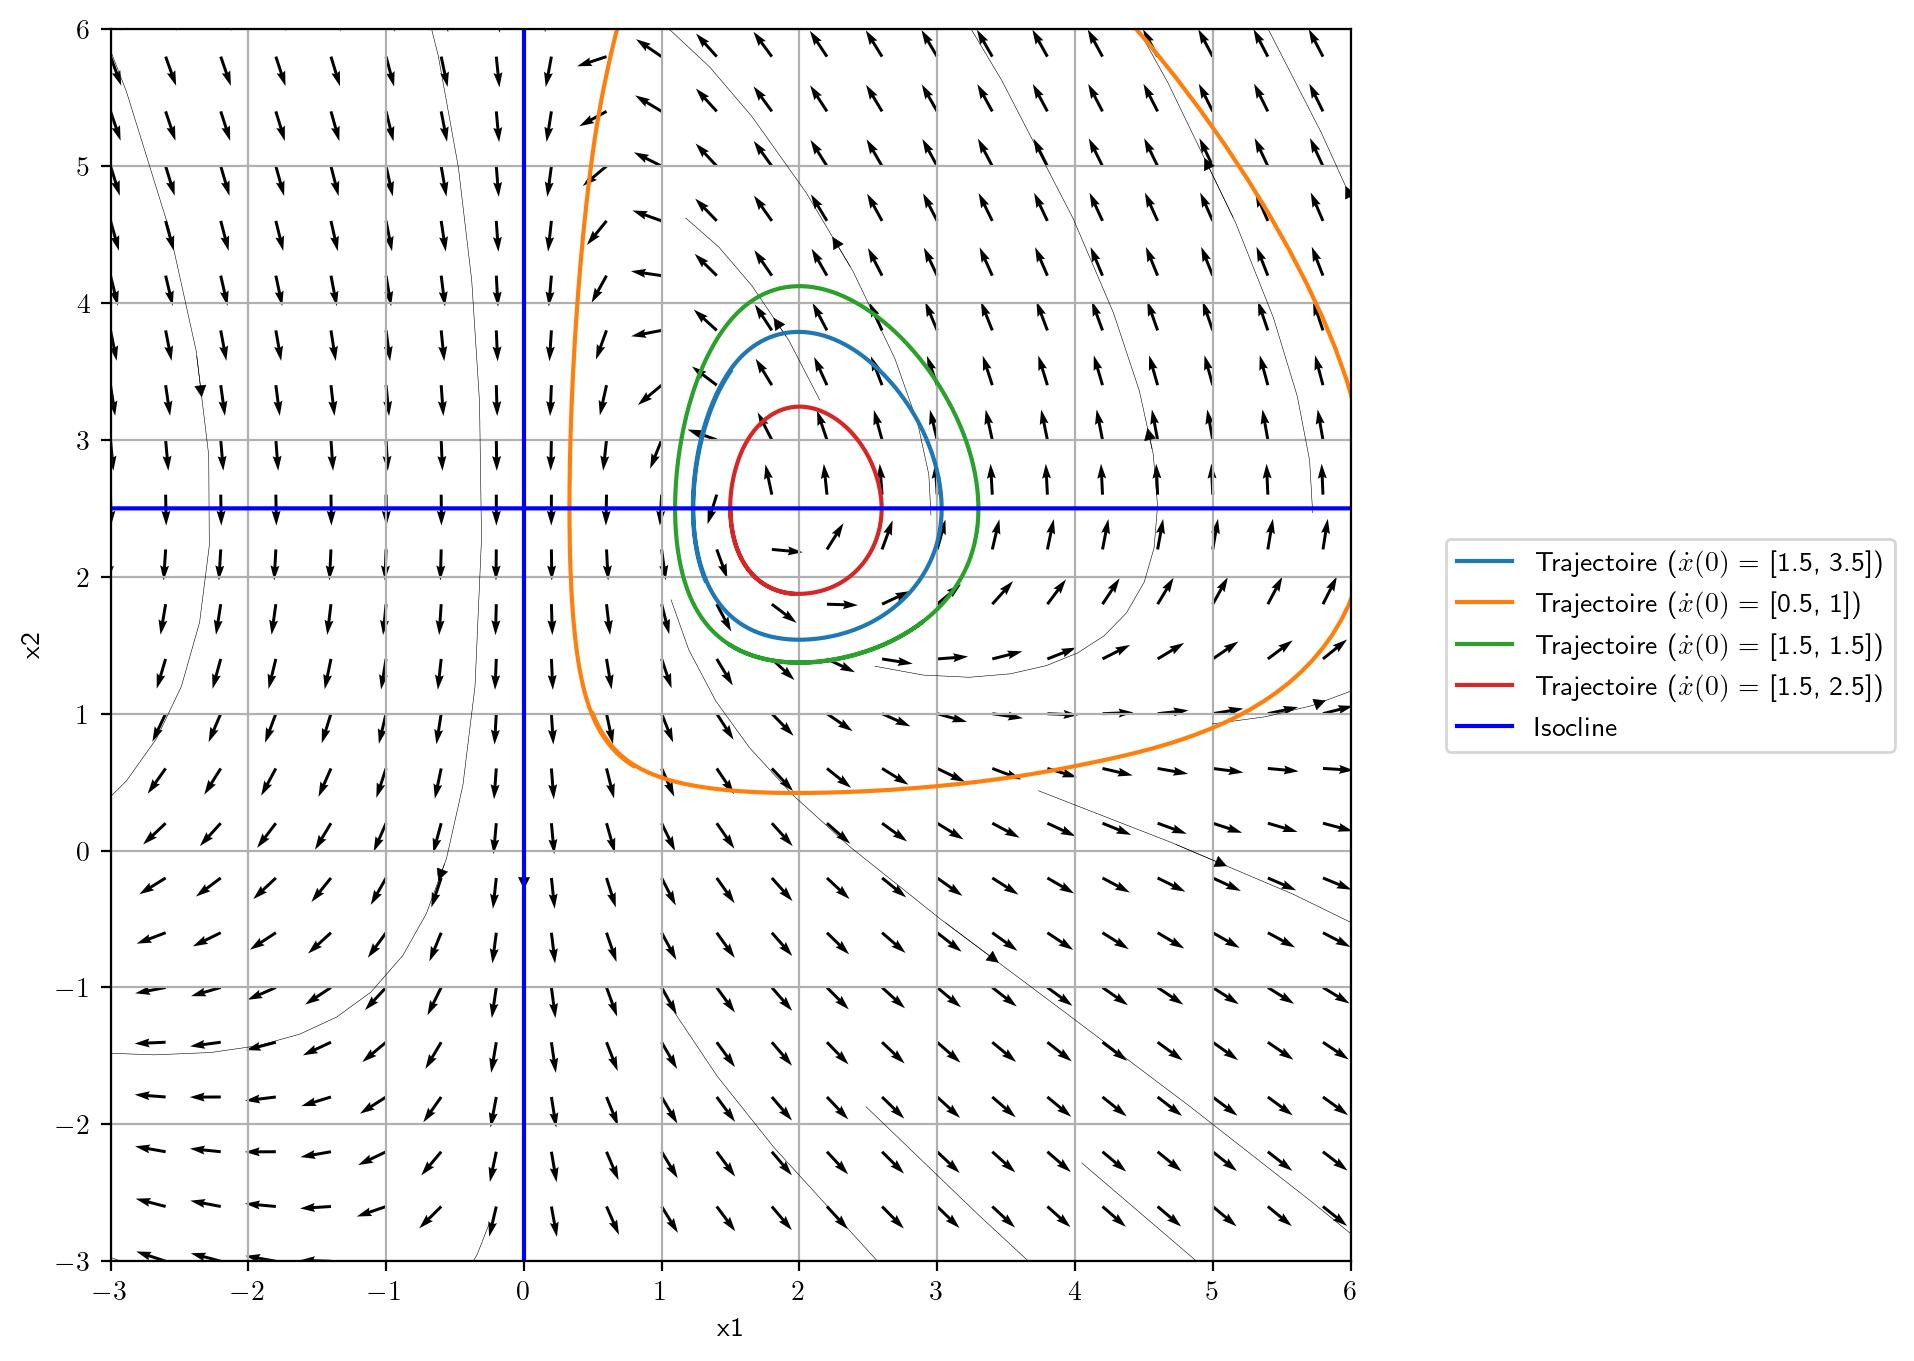
\includegraphics[width=\textwidth]{images/pdp_exercice_3_3.jpg}
                \caption{Solution numérique de l'exercice 3}
                \label{fig:pdp_exercice_3_3}
            \end{figure}
